\subsection{Bluetooth}\label{sec:bluetooth}


\subsubsection{Major Minor Vergabe}
Um die Major Minor Nummern mit dem Dojo zu benutzen wurden sie im Verlaufe des Projektes Standartisiert. Es sind Bereiche definiert für die speziellen Funktionen der Software. Die Sprachauswahl fuktioniert über solche Nummern. Beacons mit diesen Speziellen Nummeren lösen auf dem Dojo entsprechende Funktionen aus. Auf Abbildung \re{fig:Bluetooth_def_MM} sind die ersten Definitionen beschrieben. Die Nummerenräume sind so gestaltet, dass es genug Platz hat, um zusätzliche Funktionen hizuzufügen, zum Beispiel weitere Sprachen oder Zugangskontrollen.

\begin{figure}[htbp!!!!]
	\centering
	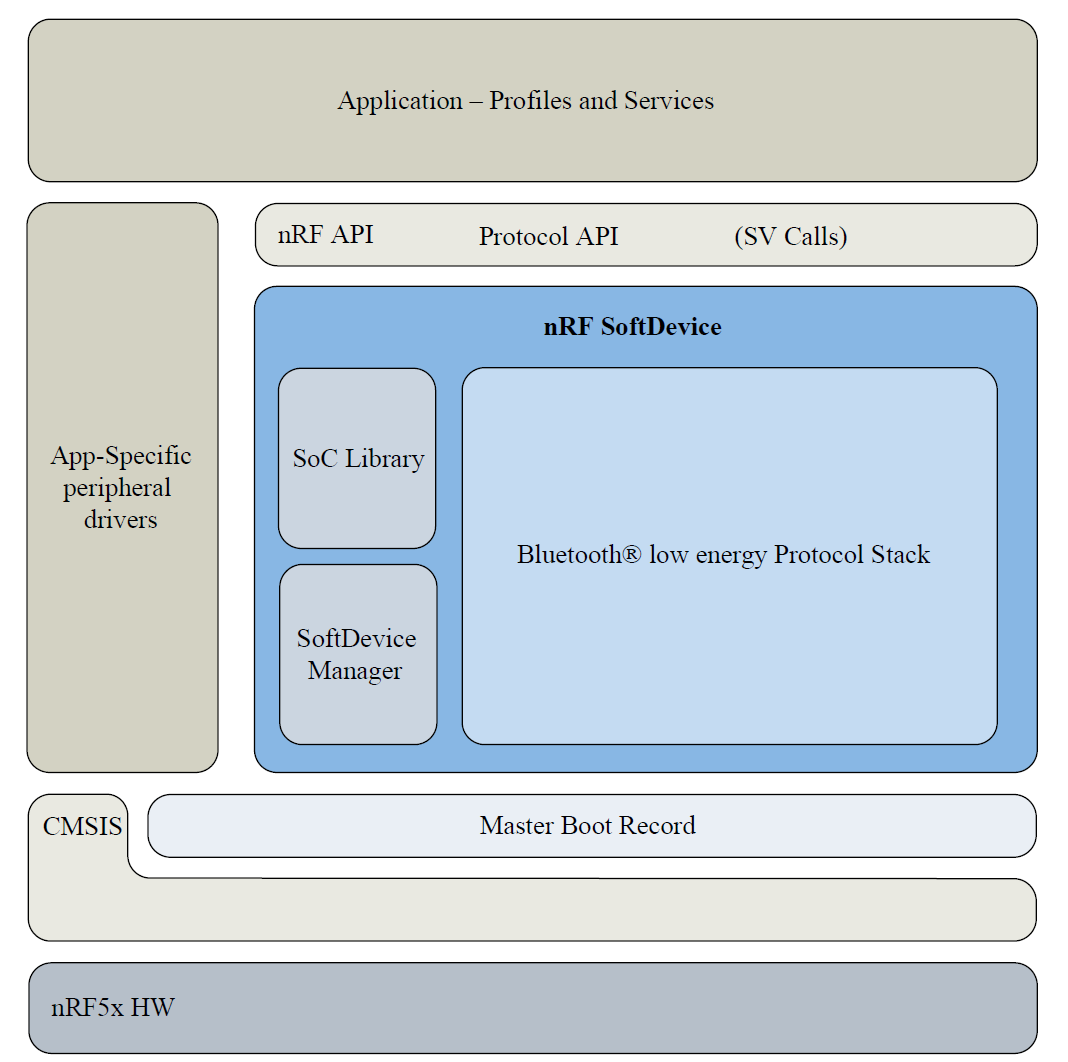
\includegraphics[width=0.7\textwidth]{Data/Software_Layers.PNG}
	\caption[Software:Definierte MM]{Default Definitionen von speziellen Major Minor Nummern.}
	\label{fig:Bluetooth_def_MM}
\end{figure}



